\documentclass[12pt]{report}
\usepackage[utf8]{inputenc}
\usepackage[russian]{babel}
%\usepackage[14pt]{extsizes}
\usepackage{listings}
\usepackage{graphicx}
\usepackage{amsmath,amsfonts,amssymb,amsthm,mathtools} 
\usepackage{pgfplots}
\usepackage{filecontents}
\usepackage{float}
\usepackage{comment}
\usepackage{indentfirst}
\usepackage{eucal}
\usepackage{enumitem}
%s\documentclass[openany]{book}
\frenchspacing

\usepackage{indentfirst} % Красная строка

\usetikzlibrary{datavisualization}
\usetikzlibrary{datavisualization.formats.functions}

\usepackage{amsmath}


% Для листинга кода:
\lstset{ %
	language=c,                 % выбор языка для подсветки (здесь это С)
	basicstyle=\small\sffamily, % размер и начертание шрифта для подсветки кода
	numbers=left,               % где поставить нумерацию строк (слева\справа)
	numberstyle=\tiny,           % размер шрифта для номеров строк
	stepnumber=1,                   % размер шага между двумя номерами строк
	numbersep=5pt,                % как далеко отстоят номера строк от подсвечиваемого кода
	showspaces=false,            % показывать или нет пробелы специальными отступами
	showstringspaces=false,      % показывать или нет пробелы в строках
	showtabs=false,             % показывать или нет табуляцию в строках
	frame=single,              % рисовать рамку вокруг кода
	tabsize=2,                 % размер табуляции по умолчанию равен 2 пробелам
	captionpos=t,              % позиция заголовка вверху [t] или внизу [b] 
	breaklines=true,           % автоматически переносить строки (да\нет)
	breakatwhitespace=false, % переносить строки только если есть пробел
	escapeinside={\#*}{*)}   % если нужно добавить комментарии в коде
}


\usepackage[left=2cm,right=2cm, top=2cm,bottom=2cm,bindingoffset=0cm]{geometry}
% Для измененных титулов глав:
\usepackage{titlesec, blindtext, color} % подключаем нужные пакеты
\definecolor{gray75}{gray}{0.75} % определяем цвет
\newcommand{\hsp}{\hspace{20pt}} % длина линии в 20pt
% titleformat определяет стиль
\titleformat{\chapter}[hang]{\Huge\bfseries}{\thechapter\hsp\textcolor{gray75}{|}\hsp}{0pt}{\Huge\bfseries}


% plot
\usepackage{pgfplots}
\usepackage{filecontents}
\usetikzlibrary{datavisualization}
\usetikzlibrary{datavisualization.formats.functions}

\begin{document}
	%\def\chaptername{} % убирает "Глава"
	\thispagestyle{empty}
	\begin{titlepage}
		\noindent \begin{minipage}{0.15\textwidth}
			
\includegraphics[width=\linewidth]{b_logo}
		\end{minipage}
		\noindent\begin{minipage}{0.9\textwidth}\centering
			\textbf{Министерство науки и высшего образования Российской Федерации}\\
			\textbf{Федеральное государственное бюджетное образовательное учреждение высшего образования}\\
			\textbf{~~~«Московский государственный технический университет имени Н.Э.~Баумана}\\
			\textbf{(национальный исследовательский университет)»}\\
			\textbf{(МГТУ им. Н.Э.~Баумана)}
		\end{minipage}
		
		\noindent\rule{18cm}{3pt}
		\newline\newline
		\noindent ФАКУЛЬТЕТ $\underline{\text{«Информатика и системы управления»}}$ \newline\newline
		\noindent КАФЕДРА $\underline{\text{«Программное обеспечение ЭВМ и информационные технологии»}}$\newline\newline\newline\newline\newline
		
		\begin{center}
			\noindent\begin{minipage}{1.1\textwidth}\centering
				\Large\textbf{  Отчет по лабораторным работам №17 - 18}\newline
				\textbf{по дисциплине <<Функциональное и логическое}\newline
				\textbf{~~~программирование>>}\newline\newline
			\end{minipage}
		\end{center}
		
		\noindent\textbf{Тема} $\underline{\text{Обработка, формирование и модификация списков на Prolog}}$\newline\newline
		\noindent\textbf{Студент} $\underline{\text{Варламова Е.А.~~~~~~~~~~~~~~~~~~~~~~~~~~~~~~~~~~~~~~~~~~~~~~~~~}}$\newline\newline
		\noindent\textbf{Группа} $\underline{\text{ИУ7-61Б~~~~~~~~~~~~~~~~~~~~~~~~~~~~~~~~~~~~~~~~~~~~~~~~~~~~~~~~~}}$\newline\newline
		\noindent\textbf{Оценка (баллы)} $\underline{\text{~~~~~~~~~~~~~~~~~~~~~~~~~~~~~~~~~~~~~~~~~~~~~~~~~~~~~~~~}}$\newline\newline
		\noindent\textbf{Преподаватель} $\underline{\text{Толпинская Н.Б., Строганов Ю. В.~~~~~~~~~}}$\newline\newline\newline
		
		\begin{center}
			\vfill
			Москва~---~\the\year
			~г.
		\end{center}
	\end{titlepage}
	

\chapter*{Лабораторная работа №17}
\section*{Постановка задачи}

\textbf{Задание:} используя хвостовую рекурсию, разработать эффективную программу (комментируя назначение аргументов), позволяющую:
\begin{enumerate}
	\item Найти длину списка (по верхнему уровню);
	\item Найти сумму элементов числового списка;
	\item Найти сумму элементов числового списка, стоящих на нечетных позициях исходного списка (нумерация от 0);
\end{enumerate}

\subsection*{Решение}
\begin{lstlisting}[language=prolog]
domains
	list = integer*

predicates
	rec_length(integer, integer, list)
	length(integer, list)

	rec_sum(integer, integer, list)
	sum(integer, list)

	rec_oddsum(integer, integer, list)
	oddsum(integer, list)

clauses
	rec_length(Res, Len, [_ | Tail]) :- NewLen = Len + 1, rec_length(Res, NewLen, Tail).
	rec_length(Res, Len, []) :- Res = Len, !.
	length(Res, List) :- rec_length(Res, 0, List).

	rec_sum(Res, Sum, [Head | Tail]) :- NewSum = Sum + Head, rec_sum(Res, NewSum, Tail).
	rec_sum(Res, Sum, []) :- Res = Sum, !.
	sum(Res, List) :- rec_sum(Res, 0, List).

	rec_oddsum(Res, Sum, [_, Head | Tail]) :- NewSum = Sum + Head, rec_oddsum(Res, NewSum, Tail).
	rec_oddsum(Res, Sum, []) :- Res = Sum, !.
	oddsum(Res, List) :- rec_oddsum(Res, 0, List).

goal
	%length(Res, [1, 2, 3, 4]).
	%sum(Res, [1, 2, 3, 4]).
	%oddsum(Res, [1, 2, 3, 4]).
\end{lstlisting}

\newpage

\textbf{Вопрос}\\

Вопрос: length(Res, [1, 2])

\begin{figure}[H]
	\centering
	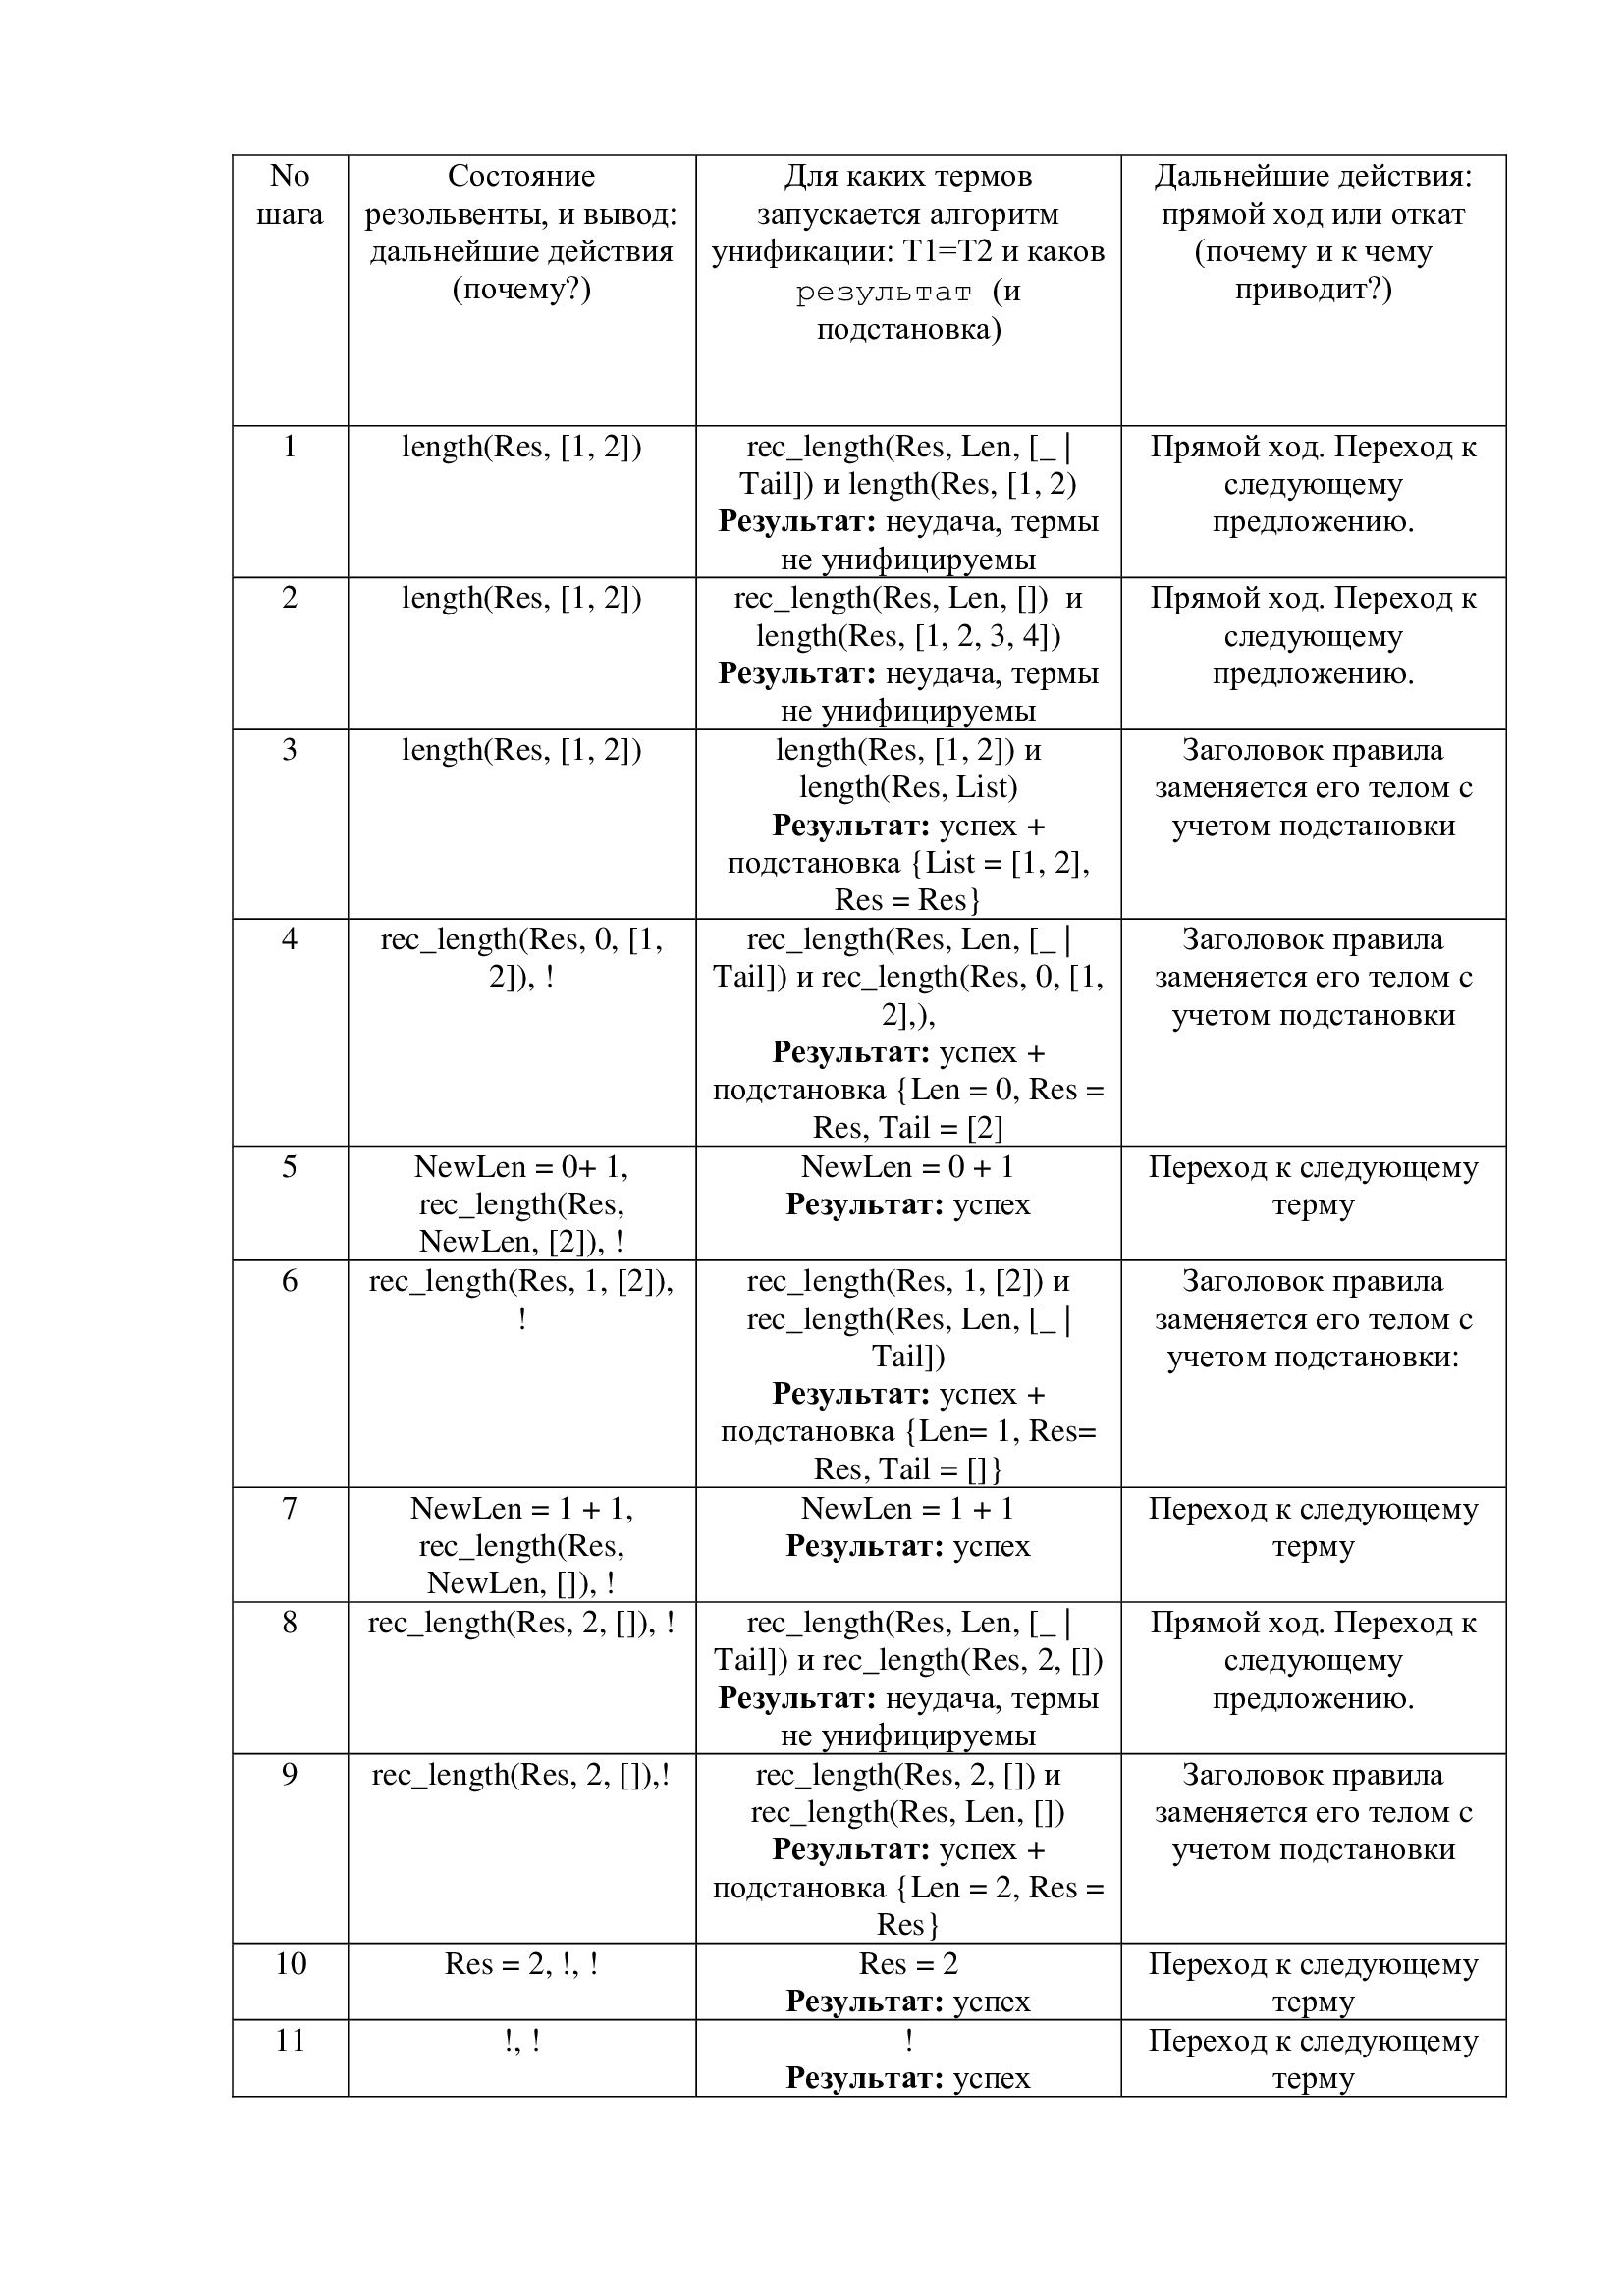
\includegraphics[scale=0.25]{lab_07_01.jpg}
	\caption{Таблица к вопросу}
	\label{d:matr_rec}
\end{figure}

\begin{figure}[H]
	\centering
	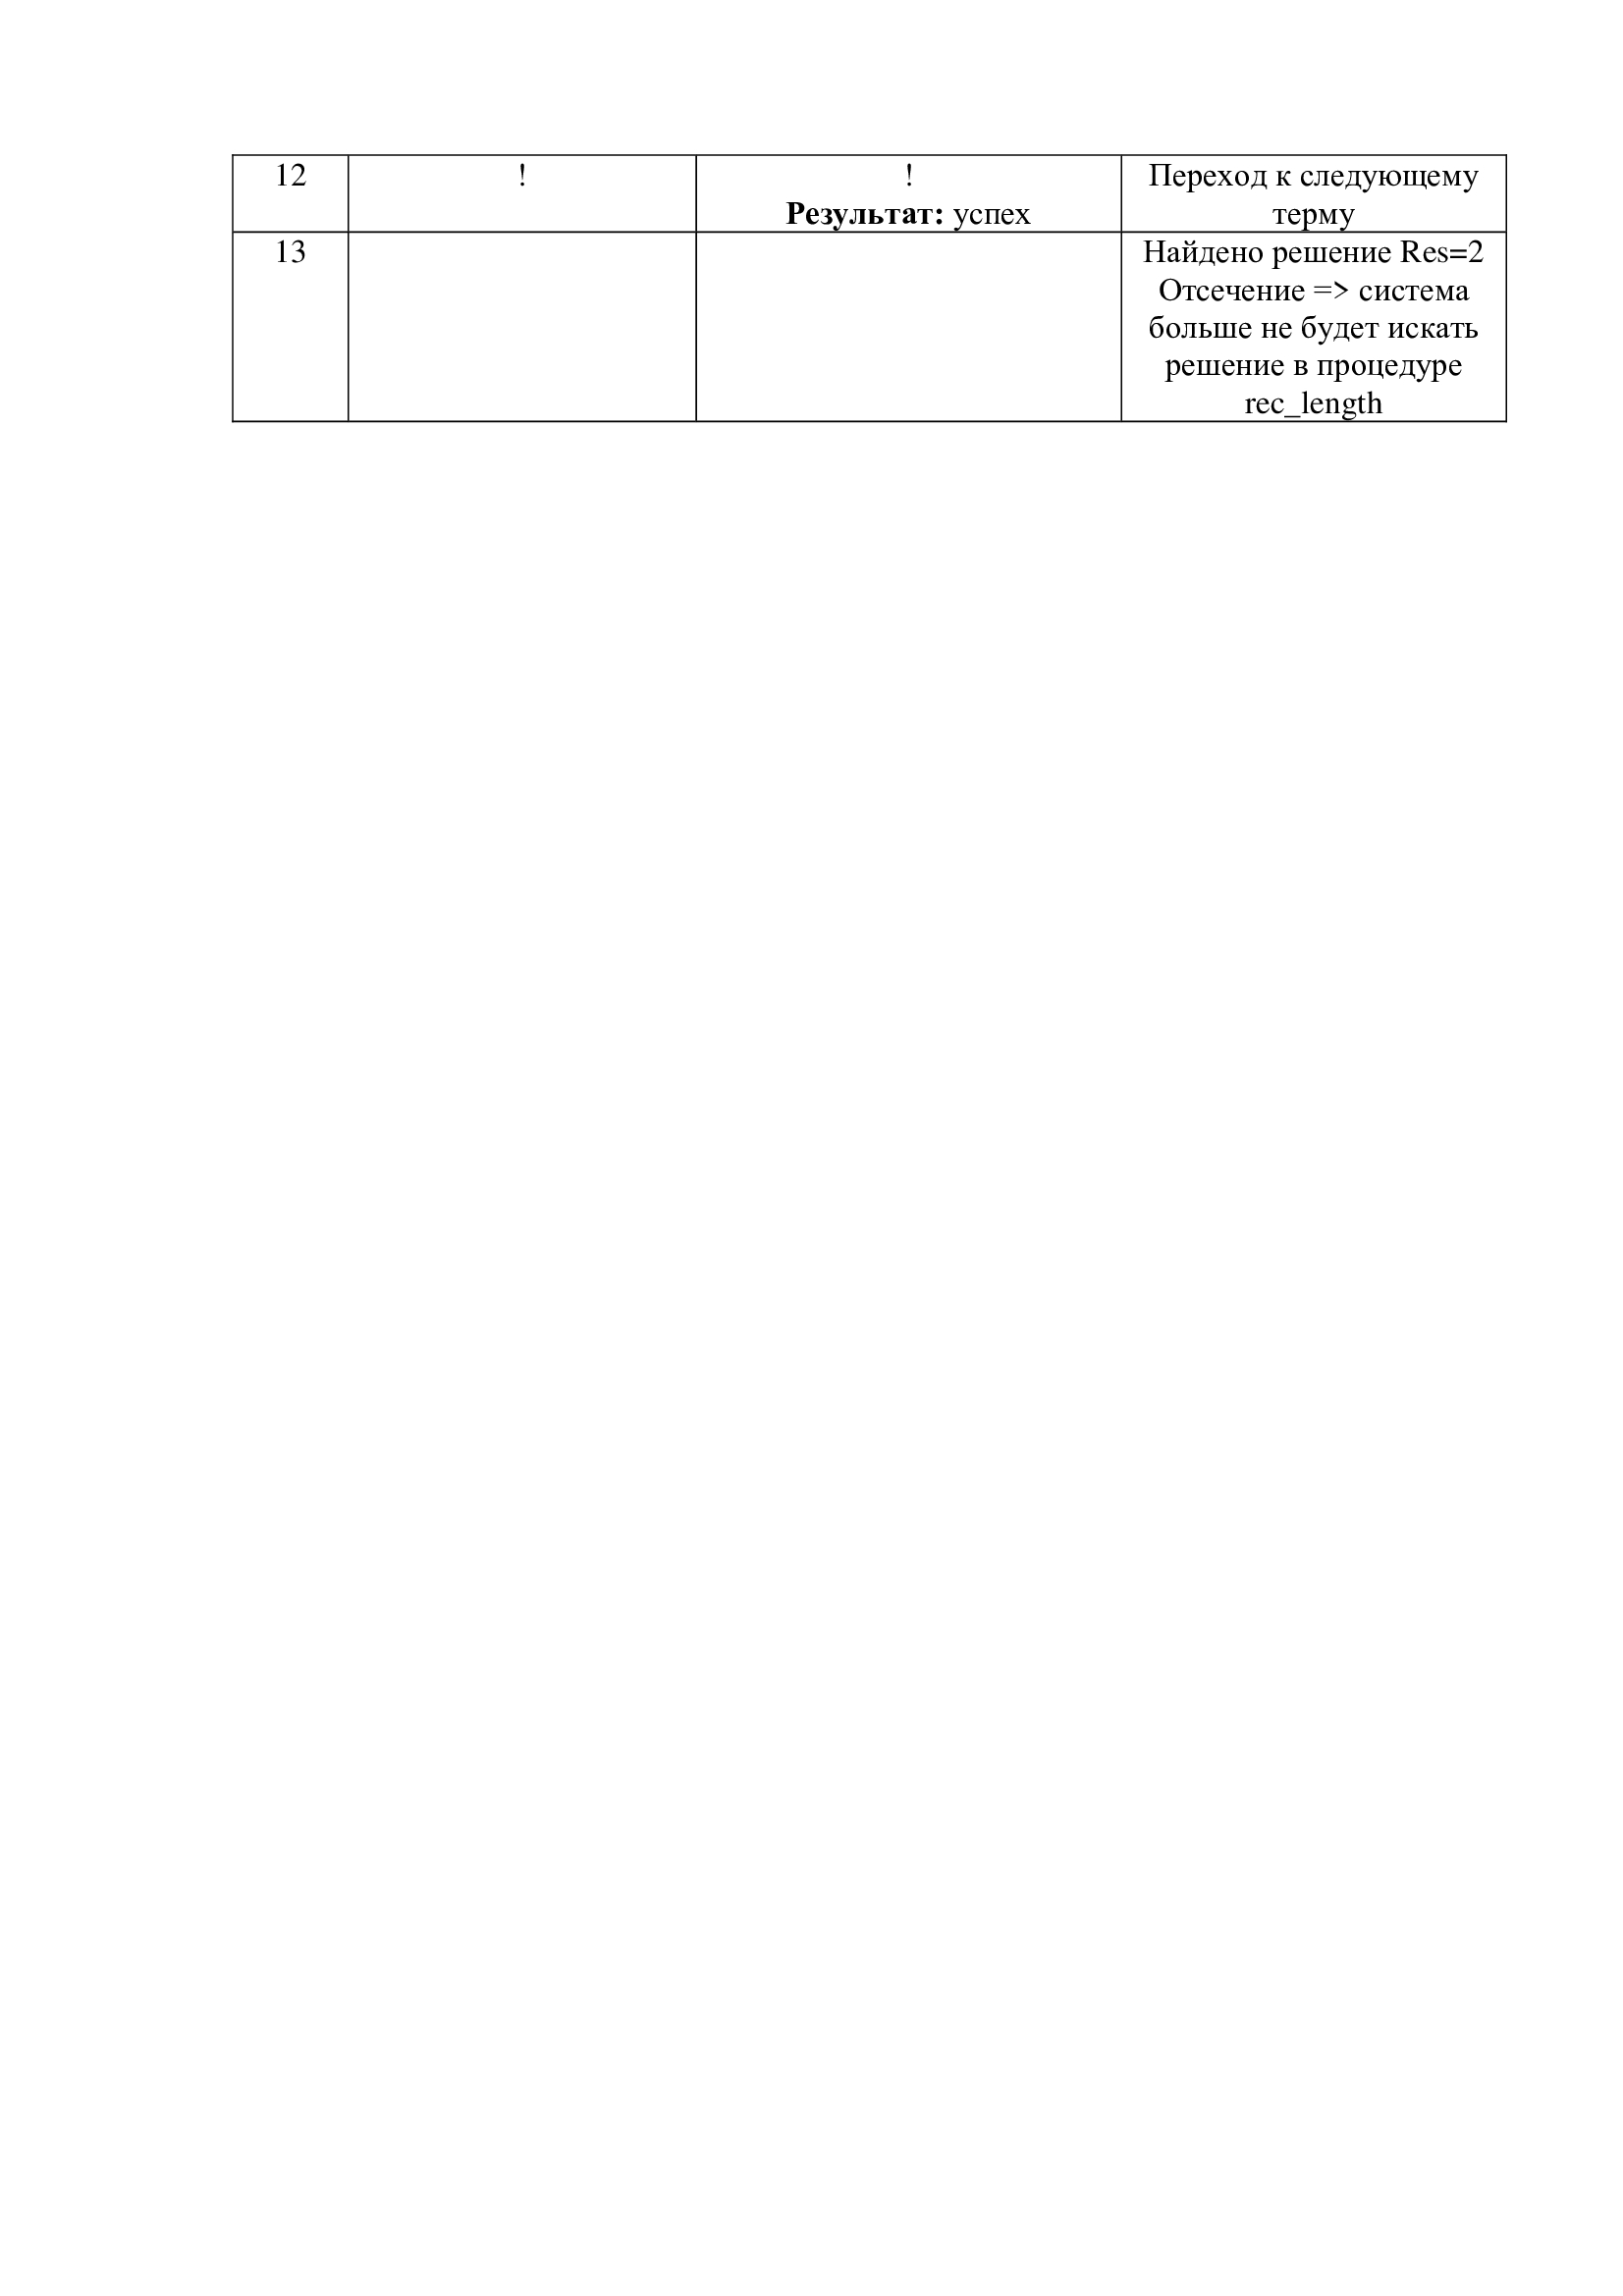
\includegraphics[scale=0.26]{lab_07_02.jpg}
	\caption{Таблица к вопросу}
	\label{d:matr_rec}
\end{figure}

\chapter*{Лабораторная работа №18}
\section*{Постановка задачи}

\textbf{Задание:} используя хвостовую рекурсию, разработать, комментируя аргументы, эффективную программу, позволяющую:
\begin{enumerate}
	\item Сформировать список из элементов числового списка, больших заданного значения;
	\item Сформировать список из элементов, стоящих на нечетных позициях исходного списка (нумерация от 0):
	\item Удалить заданный элемент из списка (один или все вхождения);
	\item Преобразовать список в множество (можно использовать ранее разработанные процедуры).
\end{enumerate}

\subsection*{Решение}
\begin{lstlisting}[language=prolog]
domains
	list = integer*

predicates
	bigger(list, integer, list)
	odd_list(list, list)
	set(list, list)
	rm_all(list, integer, list)
	rm_one(list, integer, list)

clauses
	odd_list([_, Head | Tail], [Head | ResTail]) :- odd_list(Tail, ResTail).
	odd_list([], []) :- !.
	
	bigger([Head | Tail], N, [Head | ResTail]) :- Head > N, !, bigger(Tail, N, ResTail).
	bigger([_ | Tail], N, Result) :- bigger(Tail, N, Result).
	bigger([], _, []).
	
	rm_one([Head | Tail], N, Tail) :- Head = N, !.
	rm_one([Head | Tail], N, [Head | ResList]) :- !, rm_one(Tail, N, ResList).
	rm_one([], _, []).
	
	rm_all([Head | Tail], N, [Head | ResList]) :- Head <> N, !, rm_all(Tail, N, ResList).
	rm_all([_ | Tail], N, ResList) :- rm_all(Tail, N, ResList), !.
	rm_all([], _, []).
	
	set([Head | Tail], [Head | Result]) :- rm_all(Tail, Head, Nt), !, set(Nt, Result).
	set([], []).

goal
	%bigger([1, 7, 3, 4, 5, 6, 2], 3, Result).
	%odd_list([1, 2, 3, 4, 5, 6, 7, 8], Result).
	
	%rm_one([1, 2, 3, 1, 2, 3, 1, 2, 3], 3, Result).
	%rm_all([1, 2, 3, 1, 2, 3, 1, 2, 3], 1, Result).
	
	%set([1, 2, 3, 1, 2, 3, 1, 2, 3], Result).
\end{lstlisting}

\newpage

\textbf{Вопрос}\\

Вопрос: odd\_list([1, 2, 3, 4], Result)

\begin{figure}[H]
	\centering
	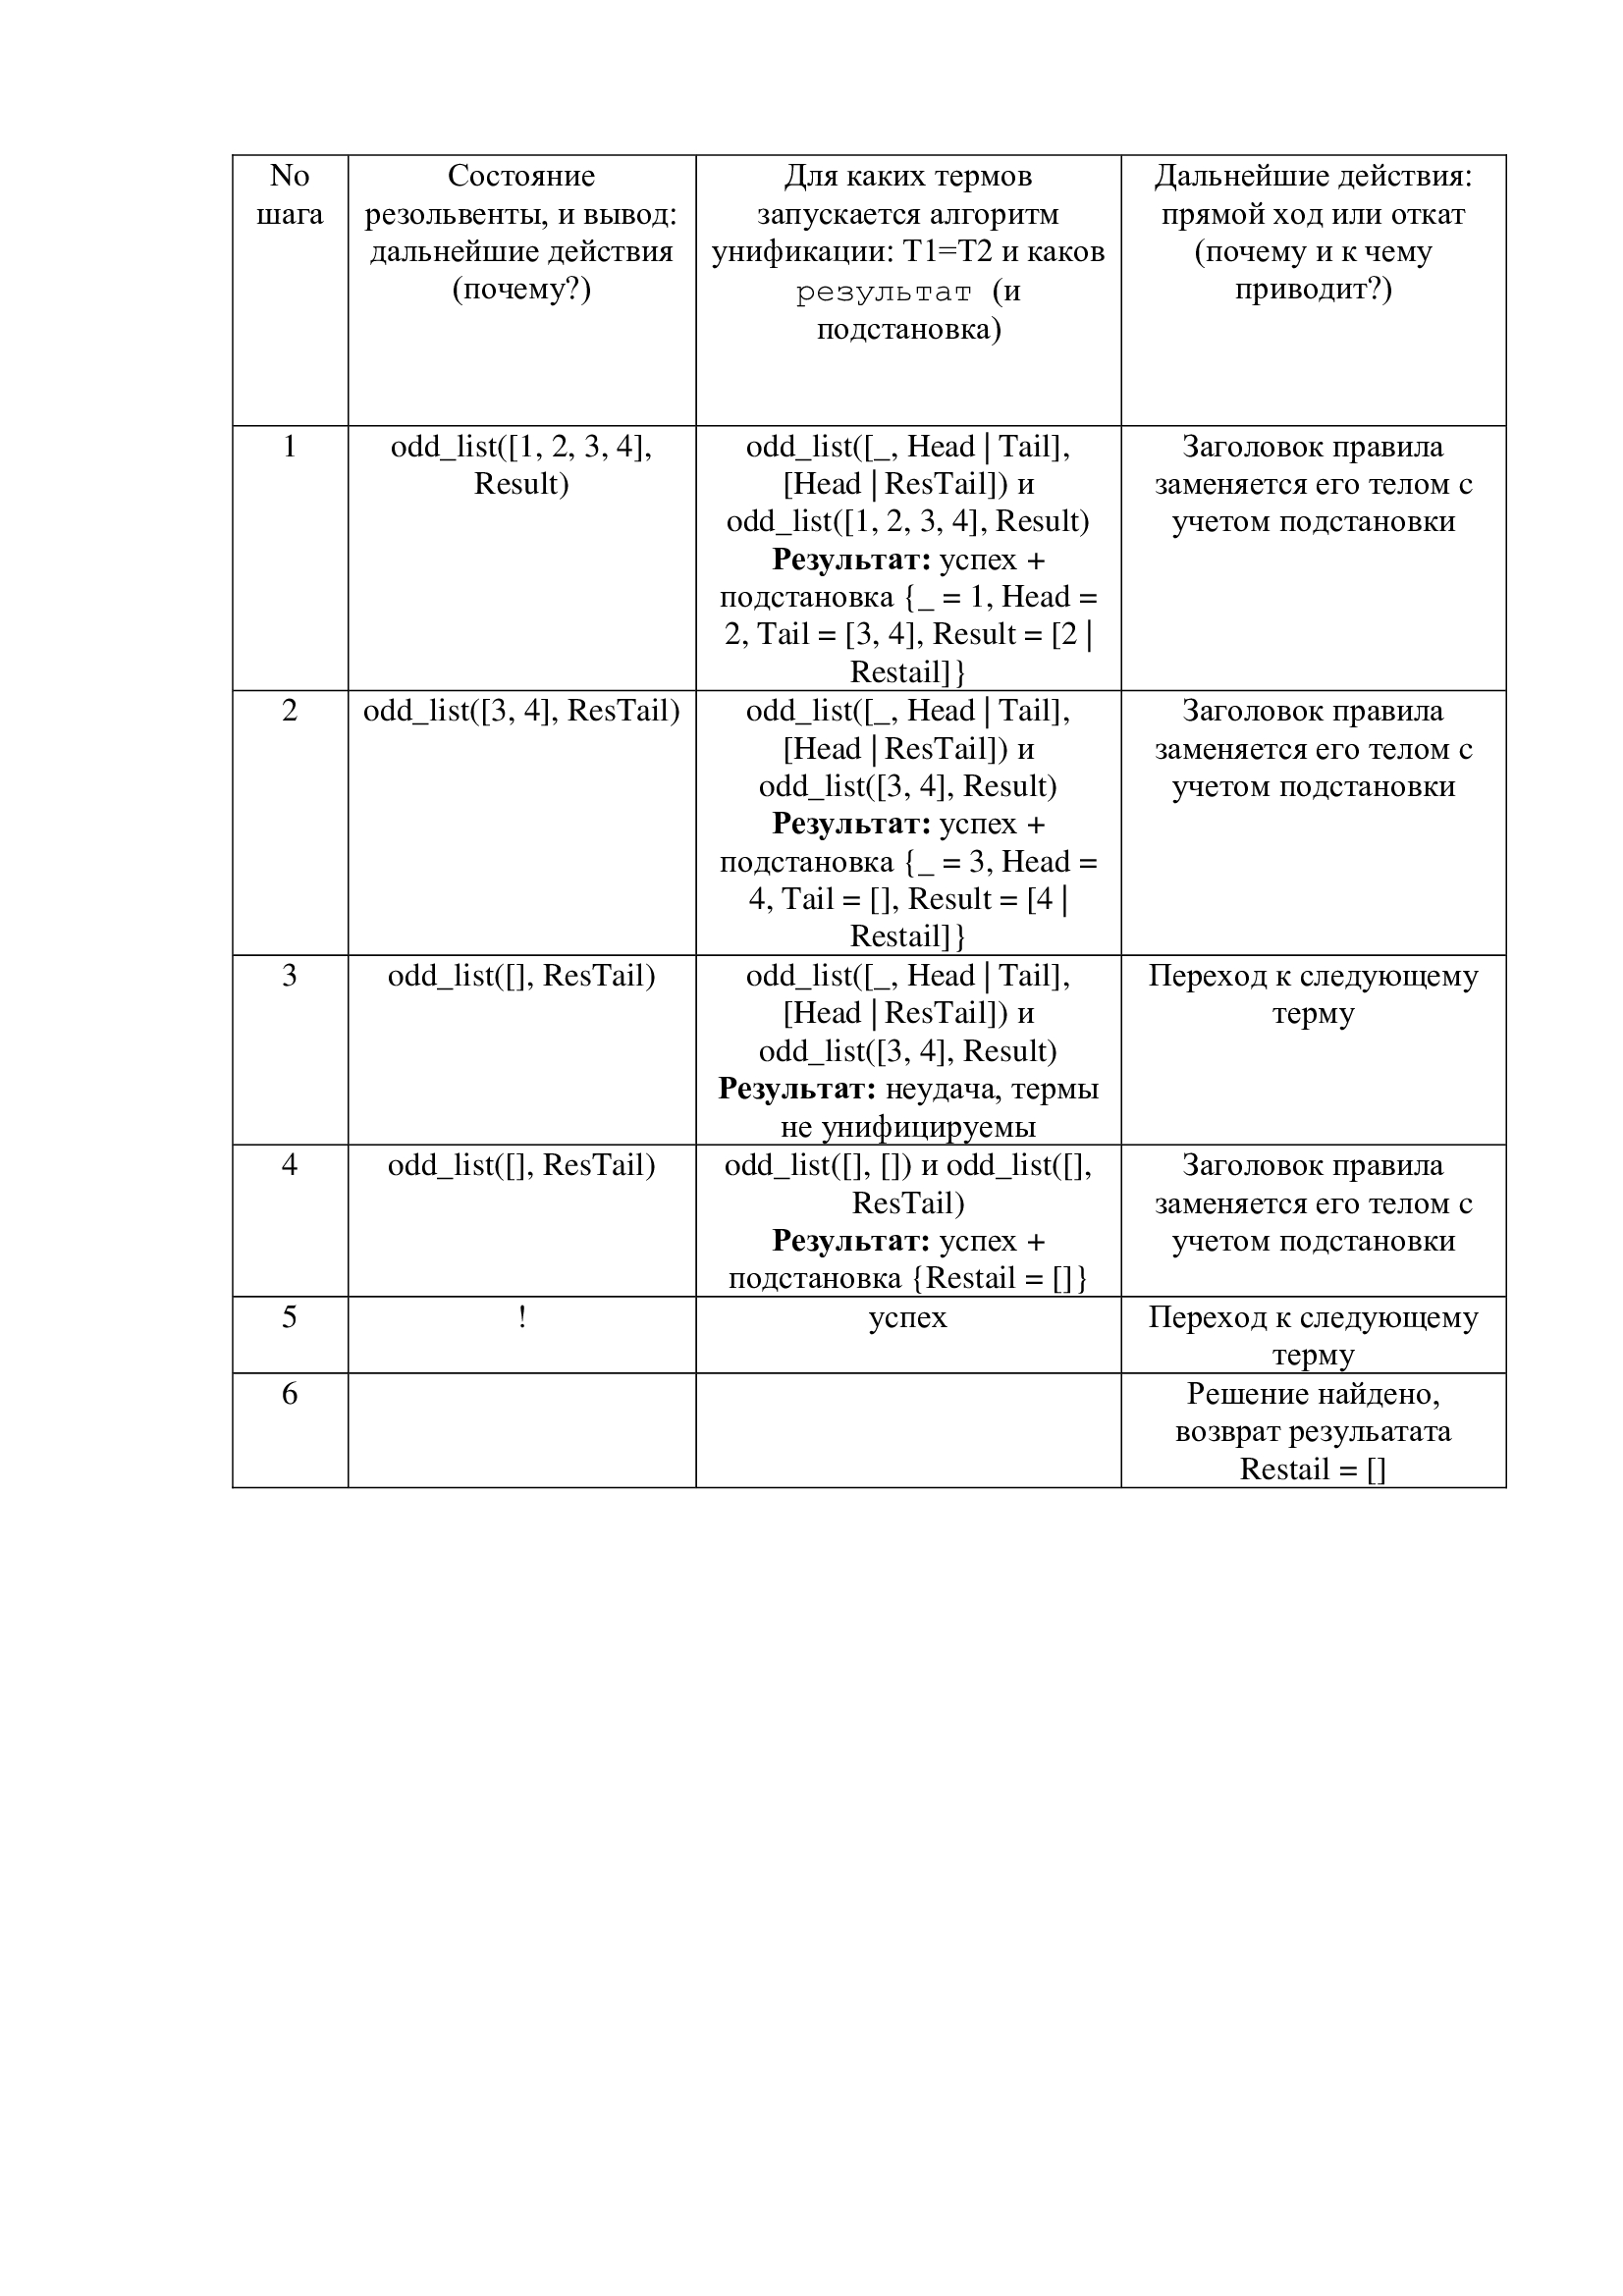
\includegraphics[scale=0.25]{lab_08_01.jpg}
	\caption{Таблица к вопросу}
	\label{d:matr_rec}
\end{figure}


\bibliographystyle{utf8gost705u}  % стилевой файл для оформления по ГОСТу
\bibliography{51-biblio}          % имя библиографической базы (bib-файла)
	
\end{document}
